\documentclass{article}

\newcommand*{\plogo}{\fbox{$\mathcal{PL}$}}

\usepackage{indentfirst}
\usepackage{anysize}
\usepackage{graphicx}
\usepackage{subfigure}
\usepackage{array}
\usepackage{makecell}
\usepackage{CJK}

\usepackage{fancyhdr}
\pagestyle{fancy}
%\usepackage[colorlinks=true,linkcolor=black,citecolor=magenta,urlcolor=red]{hyperref}
%\usepackage[all]{hypcap}

\linespread{1.2}


\marginsize{3cm}{3cm}{1cm}{1cm}
\setlength{\parindent}{2em}

\newcolumntype{L}[1]{>{\vspace{0.5em}\begin{minipage}{#1}\raggedright\let\newline\\
\arraybackslash\hspace{0pt}}m{#1}<{\end{minipage}\vspace{0.5em}}}
\newcolumntype{R}[1]{>{\vspace{0.5em}\begin{minipage}{#1}\raggedleft\let\newline\\
\arraybackslash\hspace{0pt}}m{#1}<{\end{minipage}\vspace{0.5em}}}
\newcolumntype{C}[1]{>{\vspace{0.5em}\begin{minipage}{#1}\centering\let\newline\\
\arraybackslash\hspace{0pt}}m{#1}<{\end{minipage}\vspace{0.5em}}}

%使得图片显示对应章节
\renewcommand\thefigure{\thesection.\arabic{figure}}
\makeatletter
\@addtoreset{figure}{section}
\makeatother


\begin{document}
\begin{CJK}{UTF8}{gbsn}
%页眉、页脚设置
\lhead{
	\setlength{\unitlength}{1mm}
        \begin{picture}(0,0)
        \put(0,0){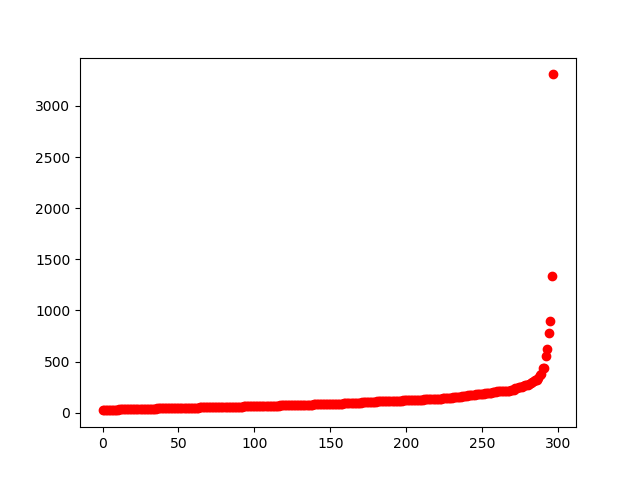
\includegraphics[width=0.7cm]{1.jpg}}
        \end{picture}
}
\chead{}
\rhead{\bfseries DAM-2018}
\lfoot{\itshape Tongji University}
\cfoot{\thepage}
\rfoot{\itshape School of Software Engineering}
\renewcommand{\headrulewidth}{0.4pt}
\renewcommand{\footrulewidth}{0.4pt}

\newcommand*{\titleGP}{\begingroup % Create the command for including the title page in the document
\centering % Center all text
\vspace*{\baselineskip} % White space at the top of the page

\rule{\textwidth}{1.6pt}\vspace*{-\baselineskip}\vspace*{2pt} % Thick horizontal line
\rule{\textwidth}{0.4pt}\\[\baselineskip] % Thin horizontal line

{\LARGE 超市数据的频繁项集挖掘 -- c问分析文档
 \\ \vspace{2em} \begin{large} 数据分析与数据挖掘 \end{large}}\\[0.2\baselineskip] % Title

\rule{\textwidth}{0.4pt}\vspace*{-\baselineskip}\vspace{3.2pt} % Thin horizontal line
\rule{\textwidth}{1.6pt}\\[\baselineskip] % Thick horizontal line

\scshape % Small caps
%周一  饶卫雄老师 \\[\baselineskip] % Tagline(s) or further description
DAM COURSE, SPRING 2018\par % Location and year

\vspace*{2\baselineskip} % Whitespace between location/year and editors

 BY \\[\baselineskip]
{\Large 1552674 李\quad 源  \par} % Editor list


\vspace{23em}
\begin{figure}[!h]
\begin{center}
  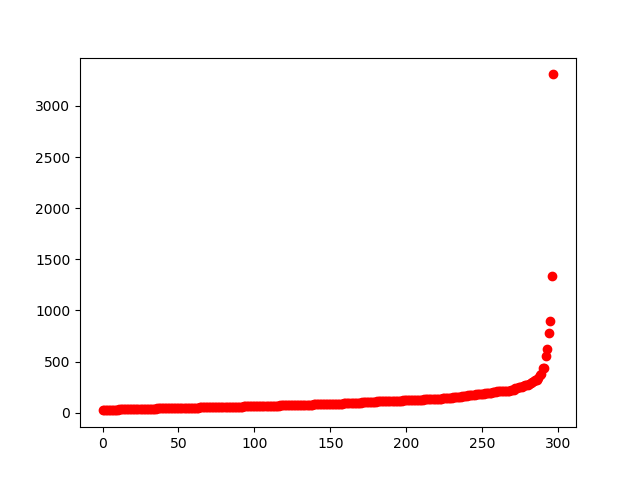
\includegraphics[width = 0.2\textwidth]{1.jpg}	
\end{center}
\end{figure}
\vfill

{\itshape Tongji University \\ School of Software Engineering \par} % Editor affiliation
\endgroup}

\titleGP % This command includes the title page
\thispagestyle{empty}
\clearpage


\section{代码运行结果}
\subsection{基于频繁项集的预测结果}
选择aii问的pluno字段输出得到的频繁项集,其中支持度前十的频繁项集作为预测,及其在后40\%中的支持度:

\begin{figure}[!h]
\begin{center}
  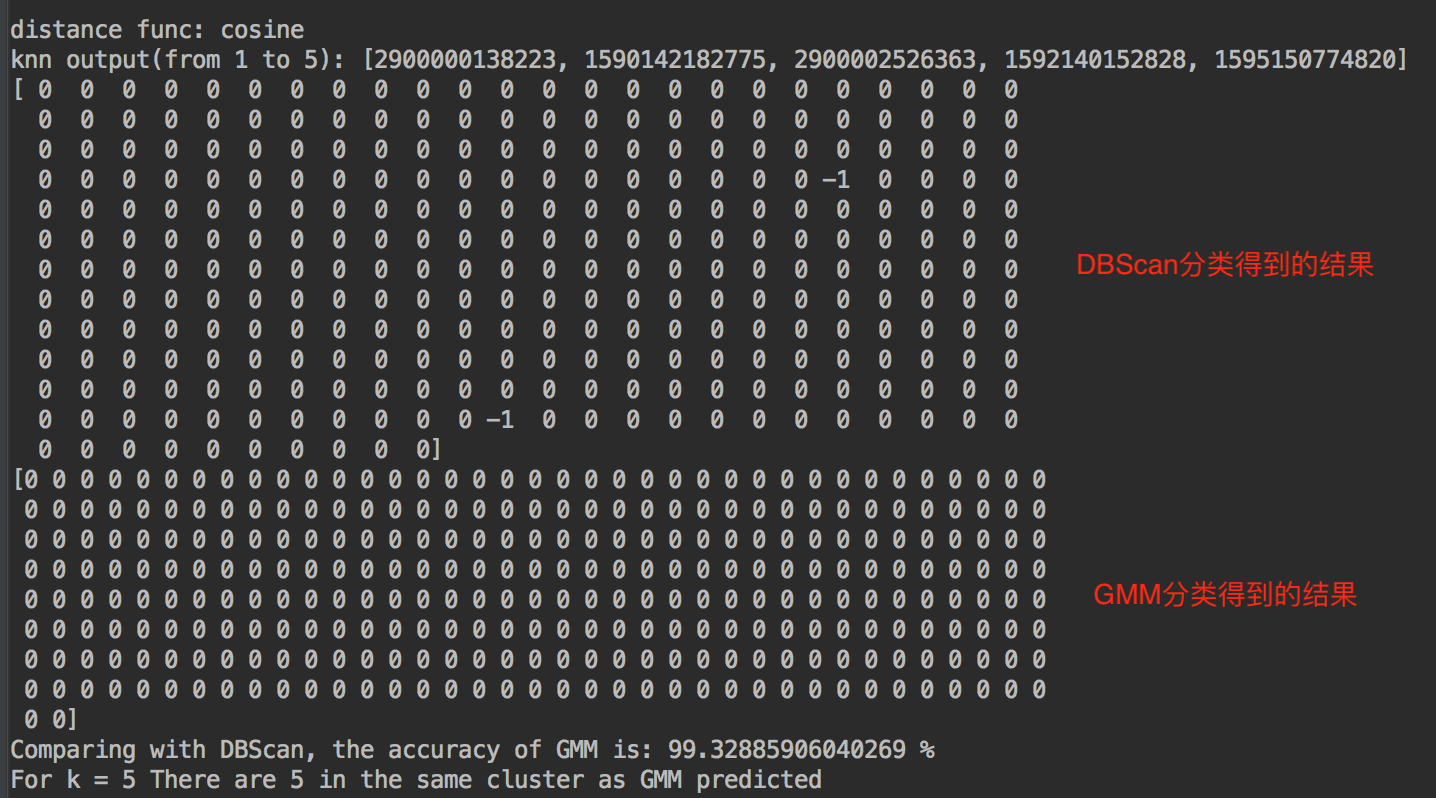
\includegraphics[width = 0.8\textwidth]{2.png}	
\end{center}
\end{figure}

选择aii问的bndno字段输出得到的频繁项集,其中支持度前十的频繁项集作为预测,及其在后40\%中的支持度:

\begin{figure}[!h]
\begin{center}
  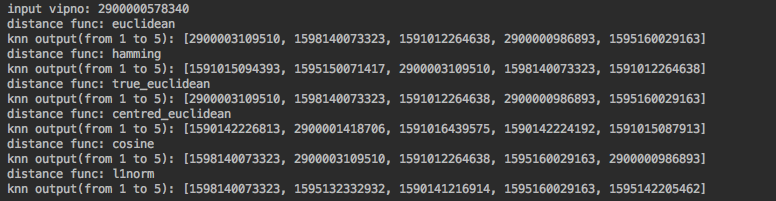
\includegraphics[width = 0.8\textwidth]{3.png}	
\end{center}
\end{figure}

\clearpage
\subsection{基于关联规则的预测结果}

选择aii问的pluno字段输出得到的频繁项集,用来生成候选的关联规则,前60\%中的置信度最高的前十关联规则作为预测,及其在后40\%中的置信度:


\begin{figure}[!h]
\begin{center}
  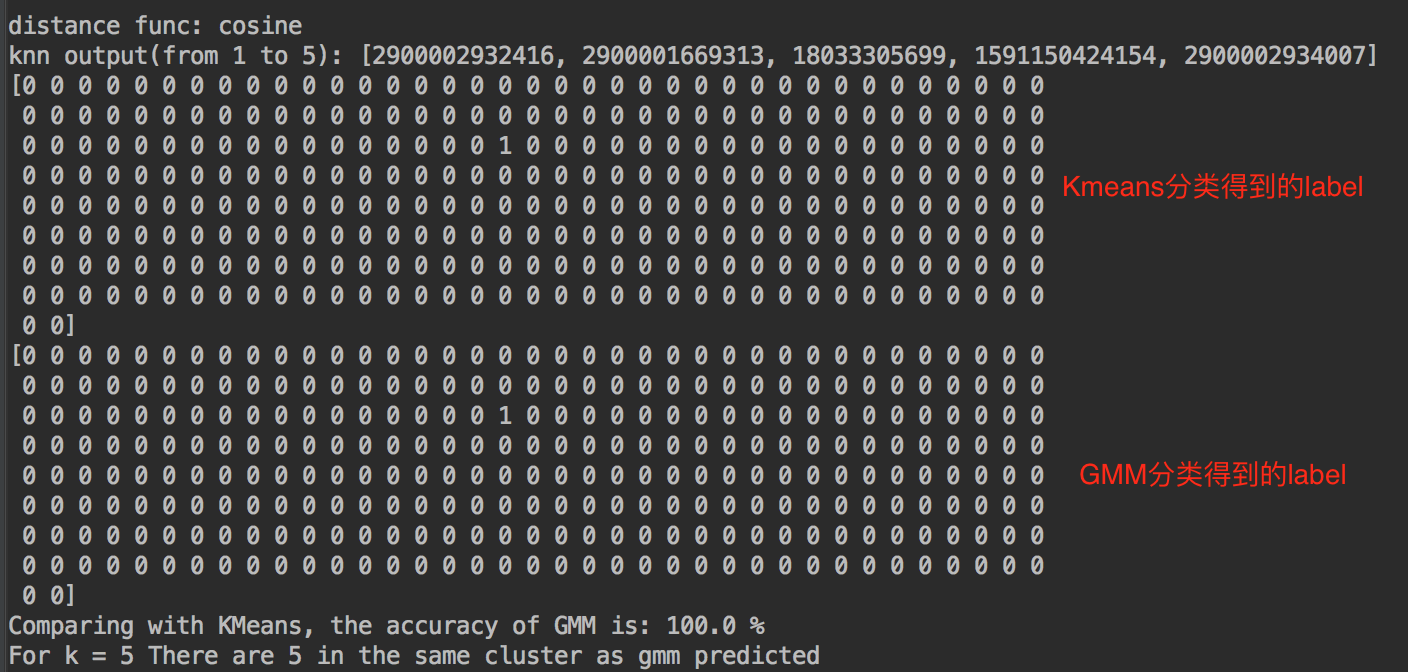
\includegraphics[width = 0.8\textwidth]{1.png}	
\end{center}
\end{figure}

选择aii问的pluno字段输出得到的频繁项集,用来生成候选的关联规则,前60\%中的置信度最高的前十关联规则作为预测,及其在后40\%中的置信度:

\begin{figure}[!h]
\begin{center}
  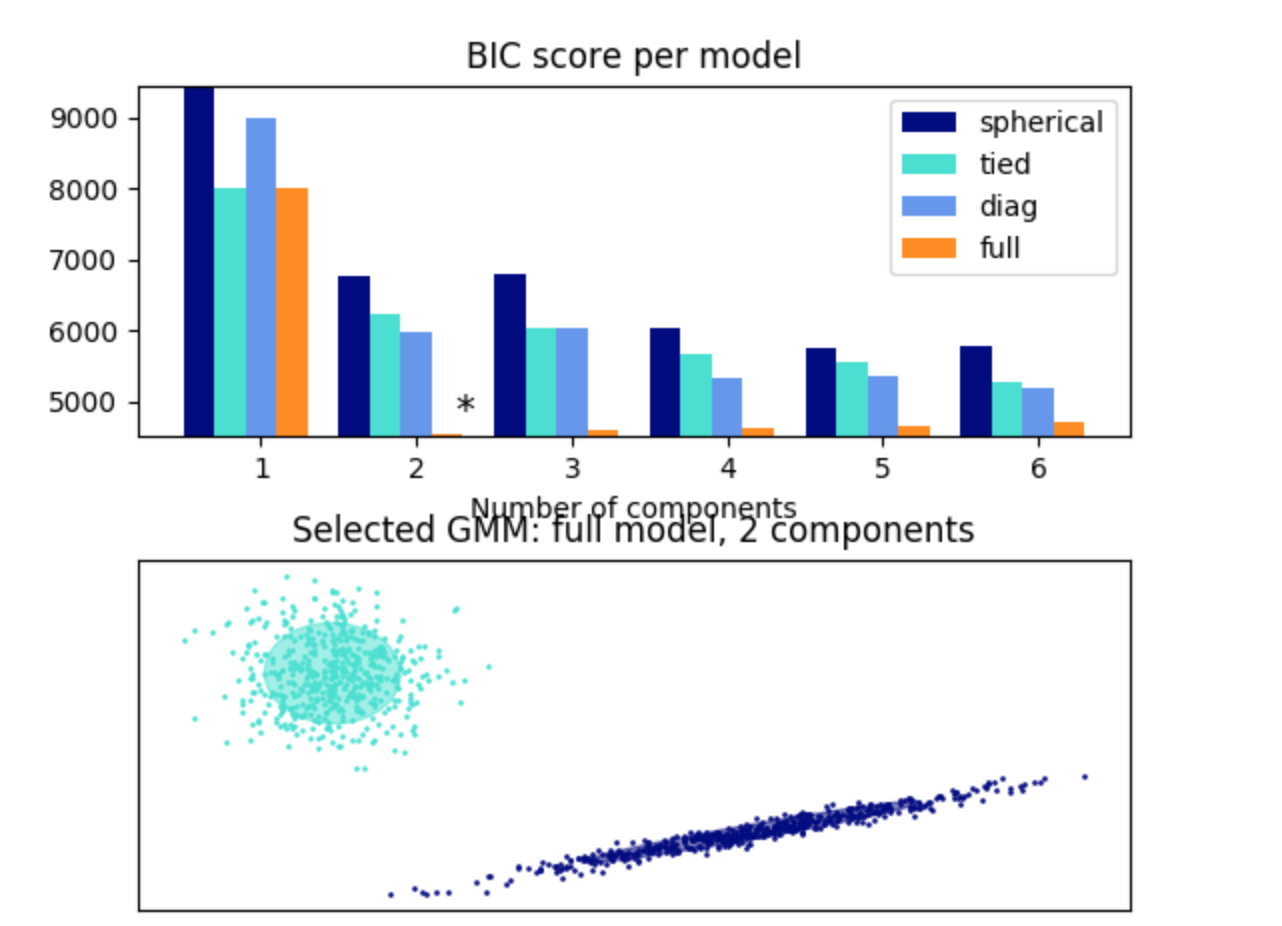
\includegraphics[width = 0.8\textwidth]{4.png}	
\end{center}
\end{figure}

80\%的关联规则都在后40\%取得了很高的置信度,说明用这些关联规则进行预测效果较好。

其他的字段得到的效果是相近的,这里为了不做一一展示了。

\section{分析讨论}
这里主要分别对两种预测方法进行分析讨论。

\subsection{基于频繁项集的预测}
在a问和b问中,我已经得到了频繁项集的输出,那么我们可以直接考虑选择支持度较高的一些频繁项集,认为是用户接下来的购买信息。

我选择了选择a、b问的字段输出得到的频繁项集,其中支持度前十的频繁项集作为预测,然后在后40\%的数据中,针对每一个用户进行评估,得到的结果如前文所示。

可以发现,前60\%中的频繁项集在后40\%中数据的支持度也比较高,并且其对排序也是相近的。那么我们可以认为,直接用生成的频繁项集来预测用户的购买信息效果是比较好的。也可以这样描述,前60\%中的频繁项集是适用于后40\%的数据。


\subsection{基于关联规则的预测}
当然,我们可以进一步通过生成关联规则来对用户的购买信息进行预测。

我们可以从频繁项集中抽取出关联规则,把几个购买信息作为作为前提,剩下的一个购买信息作为结论组成如下形式的规则:\textbf{如果用户购买了前提中的所有商品,那么他们也会想购买结论中的商品}。每一条频繁项集都可以生成几条这样的候选关联规则。

接下来,计算每条规则的置信度,这里的计算方法大致如下:

1)先创建两个字典,用来存储规则应验(正例)和规则不适用(反例)的次数。

2)遍历所有用户的购买信息,在这个过程中遍历每条关联规则。

3)逐个计算是否应验。

4)用规则应验的次数除以前提条件出现的总次数,计算每条规则的置信度。

5)排序选择置信度前十的关联规则作为预测方法。

6)在后40\%的数据上评估发现的规则在测试集上的表现。具体的输出在前文有描述。

可以发现,前60\%的数据得到的关联规则,在后40\%中也得到了很好的置信度。可以这样认为,利用关联规则来进行用户的预测,也能够取得一个很好的结果。


同时,我将trade.csv和trade\_new.csv都进行了预测,发现得到的效果是相近的。

\end{CJK}
\end{document}

